
\textbf{Bates model prices} produced by the market\!\,\footnote{
The fit uses 245 calibration cells across 7 maturities and 100 strikes,
backed by 302,943 contracts of traded volume.
The reference spot was $S_{\mathrm{ref}} = 1293.0412$,
priced under a risk-free rate of 0.15\% and a dividend rate of 2.07\%.
The intraday spot range was 1.21\%.
Fit quality is 0.53 vol points of implied-volatility RMSE,
with a relative-price RMSE of 0.104.
The Feller condition violates at this calibration,
with $2\kappa\theta - \eta^2 = -0.1921$.
} 
calibrated pricing operator:
\begin{center}
    $C_{\mathrm{Bates}}(\Theta^{\star}; S,K,\tau,w)$~\eqref{eq:bates-cf}~\eqref{eq:accept}.
\end{center}
\begin{figure}[H]
    \begin{center}
        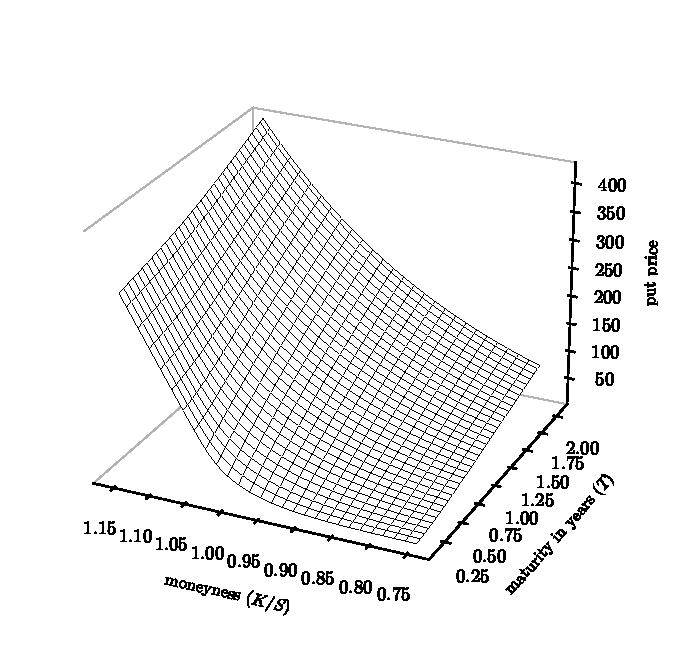
\includegraphics[width=6.25cm,keepaspectratio=true]{results/bates/surfaces/plots/tex/price_surface_puts.eps}
        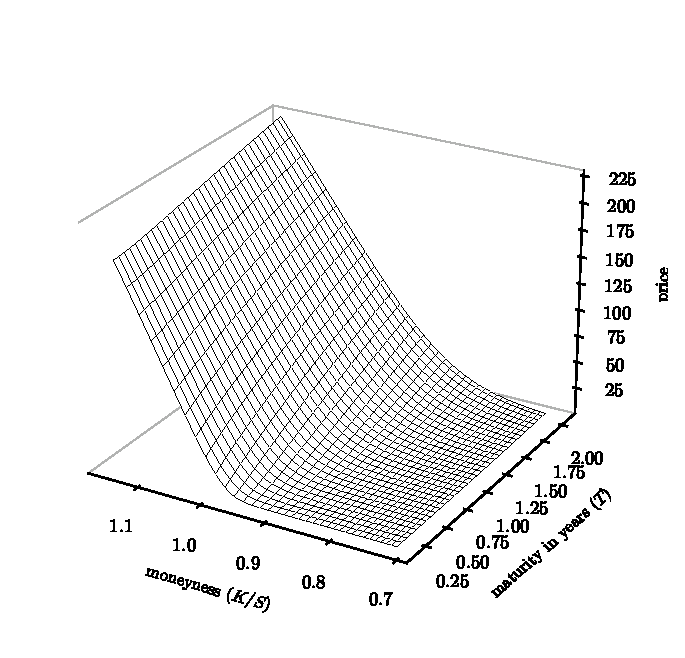
\includegraphics[width=6.25cm,keepaspectratio=true]{results/bates/surfaces/plots/tex/price_surface_calls.eps}
        \caption{Bates option prices for $S_{\mathrm{ref}}$ 1293.0412 on January 10, 2012 with $\Theta^{\star} = (0.0905,\ 0.8458,\ 0.5875,\ -0.8327,\ 0.0319, \ 0.0646, \ -0.5, \ 0.4875)$: puts wing (left) and calls wing (right).}
        \label{Fig:bates-wings}
    \end{center}
    \begin{center}
        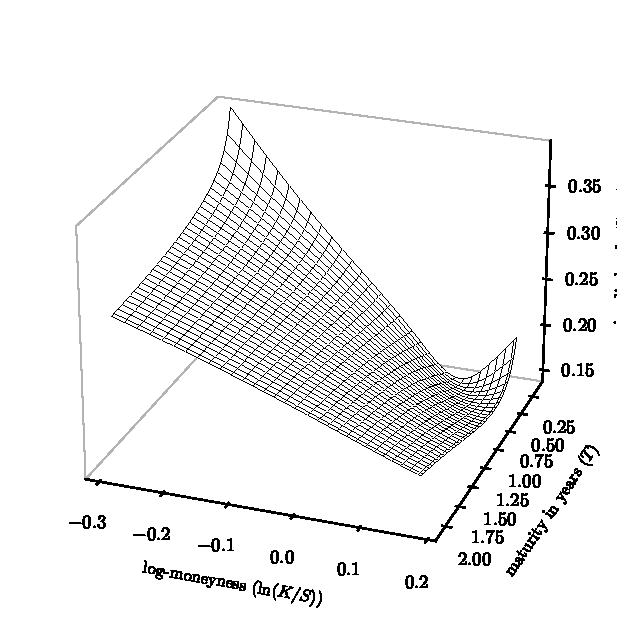
\includegraphics[width=9cm,keepaspectratio=true]{results/bates/surfaces/plots/tex/smile_surface.eps}
        \caption{\emph{Out of the money} implied volatilites from Figure~\ref{Fig:bates-wings}}
    \end{center}
\end{figure}

